\section{Usage and limitation}
We test the transfer tool with 900 million $J/\psi$ data 
which takes about 5TB disk space. 
These data are divided into 9 datasets.
It took 5 days to transfer 
these data from IHEP to JINR. The throughput is shown in 
figure \ref{fig:throughput}.
It is not very high due to the poor network connectivity.
Currently, the consistency check does not take place.
In the future version, we need to check the file is same between
the remote sites.
\begin{figure}[h]
\begin{minipage}{.49\textwidth}
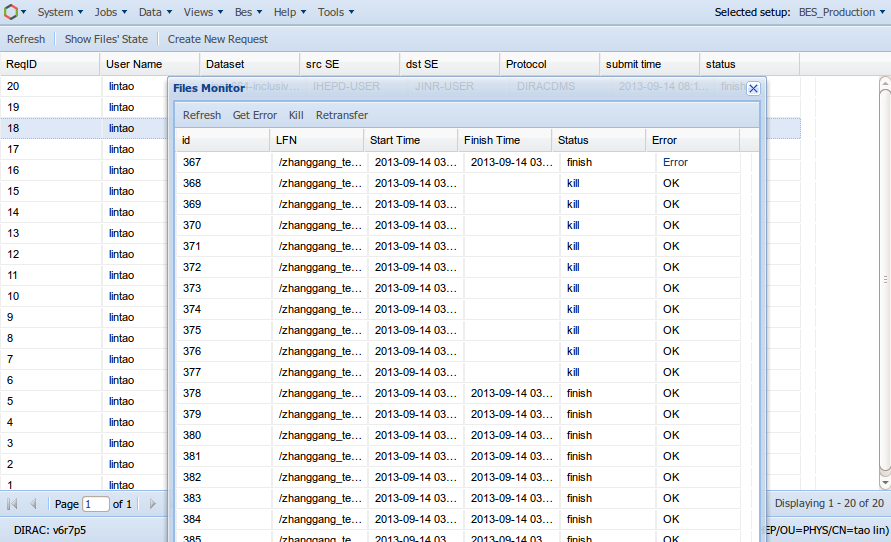
\includegraphics[width=.95\textwidth, keepaspectratio]{data/transreqlist-with-kill-retransfer.png}
\caption{\label{fig:ui}Transfer Request Management.
It shows the status of the dataset and the files in dataset.
It is in Bes$\to$Transfer$\to$Transfer Request in {\tt BESDIRAC}
web portal}
\end{minipage}
\hspace{.02\textwidth}
\begin{minipage}{.49\textwidth}
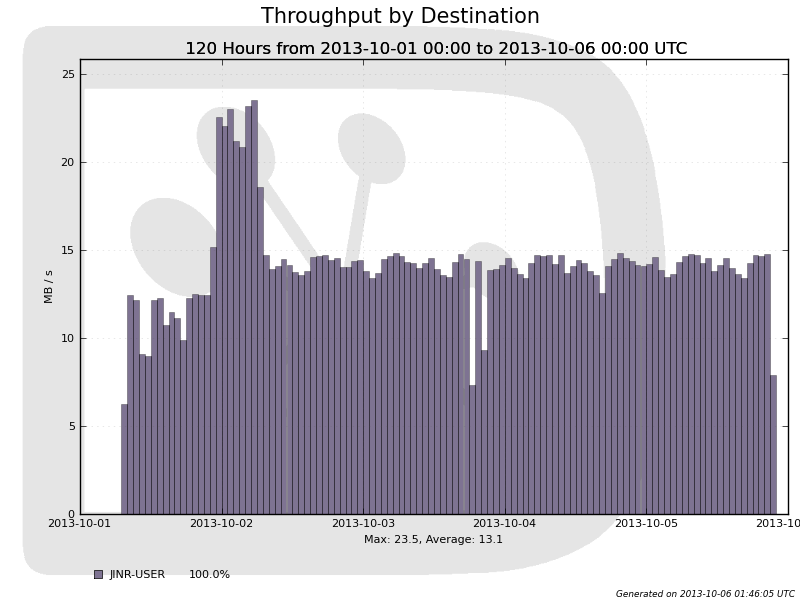
\includegraphics[width=.95\textwidth, keepaspectratio]{data/throughput-dest-1001-10-06.png}
\caption{\label{fig:throughput}Throughput from Oct.1 to Oct.6, 
average throughput is 15MB/s. This figure is generated in 
{\tt DIRAC} web portal automatically.}
\end{minipage}
\end{figure}

Now the main bottleneck of this system is the inefficiency because 
the transfer agent is deployed in one server and the maximum number of 
the workers is limited by the network bandwidth.
But this system can be easily extended.
One solution is to deploy multiple agents in different sites
so that the agents can transfer these datasets parallelly.
In order to keep up transfer status,
those transfer agents only use one database.
We will test this after several {\tt DIRAC} instances are installed.
